\documentclass{beamer}

\mode<presentation>





\usetheme{Frankfurt}%
\usecolortheme{seagull}
\logo{
\includegraphics[height=.25in]{clarksonGreen}}

\definecolor{garnet}{RGB}{136,0,0}
%\definecolor{clarksonGreen}{RGB}{0,71,28}
\definecolor{clarksonGreen}{RGB}{0,52,21}
\setbeamercolor{palette primary}{fg=clarksonGreen,bg=white}
\setbeamercolor{palette secondary}{fg=clarksonGreen,bg=white}
\setbeamercolor{palette tertiary}{fg=clarksonGreen,bg=white}
\setbeamercolor{palette quaternary}{bg=clarksonGreen,fg=white}
\setbeamercolor{block title}{fg=black,bg=black!15}
\setbeamercolor{block body}{fg=black,bg=black!10}
\setbeamercolor{titlelike}{bg=clarksonGreen,fg=white} % parent=palette quaternary}

\newcommand{\half}{\mbox{$\frac{1}{2}$}}
\newcommand{\deltat}{\mbox{$\triangle t$}}
\newcommand{\deltax}{\mbox{$\triangle x$}}
\newcommand{\deltay}{\mbox{$\triangle y$}}

\newcommand{\deriv}[2]{\frac{d}{d#2}#1}
\newcommand{\derivTwo}[2]{\frac{d^2}{d#2^2}#1}

\newcommand{\lp}{\left(}
\newcommand{\rp}{\right)}



\begin{document}

\part{Introduction}

\part{Introduction}
\lecture{Introduction}{Introduction}
\section{Introduction}

\title{Ordinary Differential Equations}
\subtitle{Introduction}
\date{27 Aug 2012}

\begin{frame}
  \titlepage
\end{frame}

\begin{frame}
  \frametitle{Outline}
  \tableofcontents[pausesection,hideothersubsections,sectionstyle=show/hide]
\end{frame}

\subsection{Syllabus}
\begin{frame}
  \frametitle{Syllabus}

  Read the syllabus! The syllabus will take precedence over any
  discrepancies here. It includes \textbf{all} of our policies. We
  will not cover them all here.

  Faculty: \\
  \begin{tabular}{l@{\hspace{3em}}l@{\hspace{3em}}l}
    Kelly Black                      & Guangming Yao    \\
    361B Science Center              & 363 Science Center   \\
    268-3831                         & 268- 6496\\
    kjblack@gmail.com                &  gyao@clarkson.edu\\ [10pt]
  \end{tabular}

\end{frame}


\begin{frame}
  \frametitle{Materials}

  \begin{itemize}
  \item {\em Differential Equations and Linear Algebra}, second
    edition
  \item Recitation manual \\
    The UPS Store, \\
    200 Market St, \\
    315.265.4565, \\
    store5986$@$theupsstore.com
  \item Turning Point Technologies ResponseCard RF LCD clicker \\
    \url{https://store.turningtechnologies.com} \\
    The Clarkson University promotional code is Z0k0.
  \end{itemize}
  
\end{frame}


\begin{frame}
  \frametitle{Test Dates}

   The tests will be given 18 September, 30 October,
  and 29 November. The exams will take place in the evenings from
  7:00pm to 8:20pm. You should bring your own pencils.  The professor
  will not have any spare materials. The location will vary depending
  on your recitation section, and your room assignments will be given
  prior to the exams.
  
\end{frame}


\begin{frame}
  \frametitle{Grading}

   \begin{tabular}[t]{rl}
    45\% & 3 Tests. \\
    20\% & Final Exam. \\
    15\% & Homework and Webwork. \\
    15\% & Quiz. \\
     5\% & Clickers
  \end{tabular}

  \begin{itemize}
  \item The right to miss a scheduled exam and take a make up exam can
    be awarded only by your professor.
  \item If for some reason you must miss an exam, you must apply in
    writing {\bf before} the exam.
  \item In case of emergency contact the professor as soon as possible
    and provide documentation to confirm why you cannot take part in
    the exam. 
  \item An unexcused absence will result in a grade of zero on the
    exam.
  \end{itemize}


  
\end{frame}


\begin{frame}
  \frametitle{Academic Accommodations}

  If you require any kind of special
  accommodation please see your professor.  Requests for academic
  accommodations must be made during the first three weeks of the
  semester, except for unusual circumstances.  Students must register
  with the Office of Accommodative Services, located in the Student
  Success Center, 110 ERC, to verify their eligibility for appropriate
  accommodations.
  
\end{frame}

\begin{frame}
  \frametitle{Clickers}

  We will start using the clickers this Friday. Each day one or more
  questions will be asked.

  You need to register your clicker. Go to our course page on moodle:
  \begin{enumerate}
  \item Choose the ``clicker ID'' option at the top of the page.
  \item Enter your clicker Device ID (found on the back of the
    clicker.)
  \item Click on the submit button.
  \item Click on the ``next'' button.
  \item Click on ``Submit all and finish.''
  \item Confirm your choice.
  \item Click on ``Finish Review'' at the bottom of the page.
  \end{enumerate}

  If you do not click on ``Finish Review'' your device ID may not be saved.
   
  
\end{frame}


\begin{frame}
  \frametitle{Recitations}

  \begin{itemize}
  \item Take place every Thursday.
  \item Will have a quiz almost every session.
  \item Some days the quiz will consist of the pre-class activity in
    your lab manual. (Random!)
  \item The recitation is where you \textbf{DO} things. It is where
    you will learn the most in this class.
  \end{itemize}
\end{frame}

\subsection{What is a Differential Equation}


\begin{frame}
  \frametitle{What is a DE?}

  Given
  \begin{eqnarray*}
    y'(x) & = & y(x),
  \end{eqnarray*}
  what is $y(x)=?$

  \begin{eqnarray*}
    \deriv{y(x)}{x} & = & y(x)
  \end{eqnarray*}

\end{frame}


\begin{frame}{Question:}
  Given
  \begin{eqnarray*}
    y'' + 3y' +2y & = & 0
  \end{eqnarray*}

  what is $y(x)$?

  \uncover<2->{
    Note: we leave often leave off the function notation.
    }

  \uncover<3->{
    Why? We are lazy!
    }

\end{frame}

\begin{frame}
  \frametitle{Notation}
  \begin{eqnarray*}
    \dot{y} & = & \deriv{y}{t} \\
    \only<2->{\ddot{y} & = & \derivTwo{y}{t} }\\
    \only<3->{y' & = & \mathrm{depends.... usually ~~} \deriv{y(x)}{x} }\\
    \only<4->{y'' & = & \derivTwo{y(x)}{x} }
  \end{eqnarray*}
\end{frame}

\begin{frame}
  \frametitle{Nomenclature}
  
  \vfill

  $\deriv{y}{x}$ - then ``ordinary differential equation.''

  \vfill

  $\frac{\partial y}{\partial x}$ - then ``partial differential
  equation.''

  \vfill

  Order is the highest number of derivatives:
  \begin{eqnarray*}
    y'' - 3 y' + 2y & = & 0, \mathrm{second~order} \\
    y'  & = & 4y, \mathrm{first~order} 
  \end{eqnarray*}

  \vfill


\end{frame}

\subsection{Modeling}


\begin{frame}
  \frametitle{Modeling}

  Why bother?

  Many ``mathematical models'' provide a relationship between rates.

  ex: Newton's Second Law, ``$\vec{F} = m \vec{a}$'' In 1 dimension:
  \begin{eqnarray*}
    m\mathrm{~(acceleration)} & = & \sum_i \lp F_x \rp_i, \\
    m \ddot{x} & = & \sum_i \lp f_x \rp_i
  \end{eqnarray*}

  
\end{frame}


\begin{frame}
  \frametitle{Circuit}
  
  The voltage across a resistor is proportional to the current flowing
  through it.

  \only<2->
  {
    There is some number, R, where
    \begin{eqnarray*}
      V & = & IR
    \end{eqnarray*}
  }
\end{frame}

\begin{frame}
  \frametitle{Proportionality}
  
  If $a$ is proportional to $b$ then there is a constant, $k$, where 
  \begin{eqnarray*}
    a  & = & k \cdot b
  \end{eqnarray*}

  if $a$ is inversely proportional to $b$ then there is a constant $c$
  where 
  \begin{eqnarray*}
    a & = & c \frac{1}{b}
  \end{eqnarray*}
\end{frame}

\begin{frame}
  \frametitle{Example - Newton's Law of Cooling}

  The rate of change of the temperature of an object is proportional
  to the difference between the object and its surroundings (the
  ambient temperature).

  \uncover<2->
  {

    Define:
    \begin{itemize}
    \item $T(t)$ is the temperature at a time $t$.
    \item $A$ is the ambient temperature (the temperature of the
      surroundings).
    \item The rate of change of the temperature is $\frac{dT(t)}{dt}$.
    \end{itemize}

  }

  \uncover<3->
  {

    There is some constant number, $k$, where 
    \begin{eqnarray*}
      \frac{dT(t)}{dt} & = & -k (T-A).
    \end{eqnarray*}

  }


\end{frame}


\begin{frame}
  \frametitle{Newton's Law of Cooling}

  The rate of change of the temperature of an object is proportional
  to the difference between the object and its surroundings (the
  ambient temperature).

    There is some constant number, $k$, where 
    \begin{eqnarray*}
      \frac{dT(t)}{dt} & = & -k (T-A).
    \end{eqnarray*}

    Question: What is the temperature at any given time?

\end{frame}


% LocalWords:  Clarkson pausesection hideothersubsections sectionstyle Yao
% LocalWords:  Guangming ResponseCard Webwork moodle


\part{Solutions to DEs}

\part{Solutions-to-DEs}
\lecture{Solutions to DEs}{Solutions-to-DEs}


\title{Ordinary Differential Equations}
\subtitle{Math 232 - Week 1, Day 2}

\author{Kelly Black}
\institute{Clarkson University}
\date{30 Aug 2011}

\begin{frame}
  \titlepage
\end{frame}

\begin{frame}
  \frametitle{Outline}
  \tableofcontents[pausesection,hideallsubsections]
\end{frame}


\section{Solutions to DEs}


\begin{frame}
  \frametitle{What is a solution to a DE?}

  \begin{eqnarray*}
    y' & = & y
  \end{eqnarray*}

  Solution: $y=3e^t$

  \uncover<2->{
    Check: 
    \begin{eqnarray*}
      y' & = & 3e^t \\
      y  & = & 3e^t
    \end{eqnarray*}

    The same!
  }

\end{frame}


\begin{frame}
  \frametitle{What is a solution to a DE?}

  \begin{eqnarray*}
    y' & = & y
  \end{eqnarray*}

  Solution: $y=2e^t$

  \uncover<2->{
    Check: 
    \begin{eqnarray*}
      y' & = & 2e^t \\
      y  & = & 2e^t
    \end{eqnarray*}

    The same!
  }


\end{frame}


\begin{frame}
  \frametitle{What is a solution to a DE?}

  \begin{eqnarray*}
    y' & = & y, \\
    y(0) & = & 1
  \end{eqnarray*}

  Neither is a solution! 

  \uncover<2->{
    Solution: $y=e^t$

    Check: 
    \begin{eqnarray*}
      y' & = & e^t \\
      y  & = & e^t \\
      y(0) & = & 1
    \end{eqnarray*}

    This is the solution.
  }

\end{frame}


\begin{frame}
  \frametitle{What is a solution to a DE?}

  Show that 
  \begin{eqnarray*}
    y & = & 3 e^{2t} - \half
  \end{eqnarray*}
  is a solution to
  \begin{eqnarray*}
    y' & = & 2y + 1.
  \end{eqnarray*}

  \uncover<2->{
    \begin{eqnarray*}
      y' & = & 6 e^{2t} \\
      2y+1 & = & 2(3 e^{2t} - \half) +1 \\
      & = & 6 e^{2t}
    \end{eqnarray*}
  }


\end{frame}


\begin{frame}
  \frametitle{What is a solution to a DE?}

  Show that 
  \begin{eqnarray*}
    y & = & \half e^{2t} - \half
  \end{eqnarray*}
  is a solution to
  \begin{eqnarray*}
    y' & = & 2y + 1, \\
    y(0) & = & 0.
  \end{eqnarray*}

  \uncover<2->{
    \begin{eqnarray*}
      y' & = & e^{2t} \\
      2y+1 & = & 2(\half e^{2t} - \half) +1 \\
      & = & e^{2t} \\
      y(0) & = & 0
    \end{eqnarray*}
  }



\end{frame}


\section{Slope Fields}

\begin{frame}
  \frametitle{What is the derivative?}

  The derivative is the slope of the tangent line.

  \begin{tabular}{lll}
    if y'=2 & slope=2 & (inc) \\
    if y'=3 & slope=3 & (inc) \\
    if y'=-2 & slope=-2 & (dec) \\
  \end{tabular}


\end{frame}


\begin{frame}
  \frametitle{Example}

  \begin{eqnarray*}
    y' & = & 5t + 3, \\
    \int y' ~ dt & = & \int 5t + 3 ~ dt \\
    \uncover<2->{y & = & \frac{5}{2} t^2 + 3t + C}
  \end{eqnarray*}

  We get a ``family of solutions.'' 

  If $y(0)=2$ then
  \begin{eqnarray*}
    y(0) & = & \frac{5}{2} (0)^2 + 3(0) + C, \\
    2    & = & C
  \end{eqnarray*}


\end{frame}


\begin{frame}
  \frametitle{Slope Fields}

  Given the differential equation can we predict the \textit{general
    behavior} of the solution? (Qualitative behavior)

  If we have 
  \begin{eqnarray*}
    y' & = & f(t,y),
  \end{eqnarray*}
  then if we know that the function goes through a point, $t=a$ and
  $y(a)=v$, then we can calculate the slope of the tangent line.

\end{frame}


\begin{frame}
  \frametitle{Example}

  \vspace*{-4em}

  \begin{eqnarray*}
    y' & = & 2y
  \end{eqnarray*}

  At $t=3$ if you happen to know that $y=4$ then the slope is 2(4)=8.

  At $t=3$ if you happen to know that $y=5$ then the slope is 2(5)=10.

  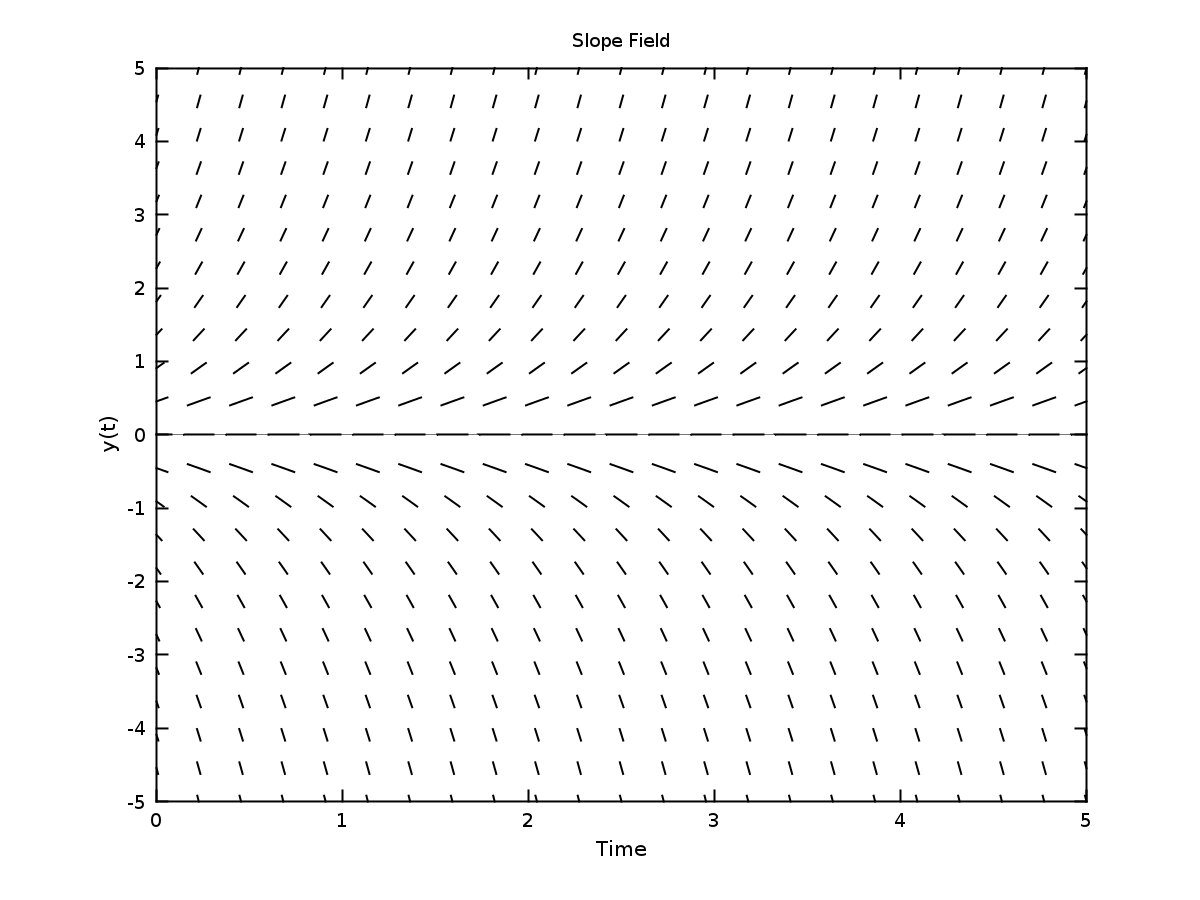
\includegraphics[height=4cm]{week1Day2SlopeField}

  A direction field is a collection of segments that indicate the
  tangent lines. 
  
\end{frame}


\begin{frame}
  \frametitle{Example}

  \vspace*{-4em}

  \begin{eqnarray*}
    y' & = & y - t
  \end{eqnarray*}

  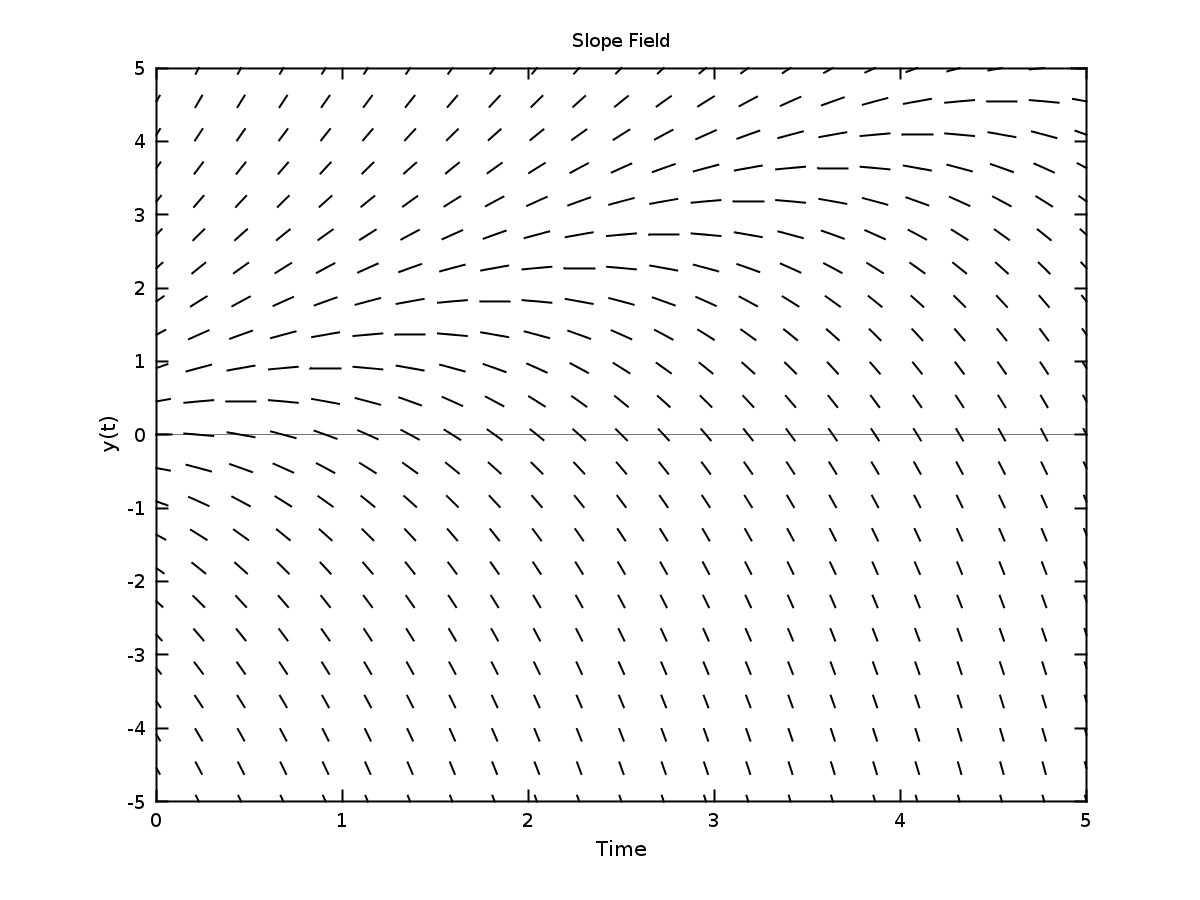
\includegraphics[height=5cm]{week1Day2SlopeField2}

  Tools:
  \begin{itemize}
  \item A ``stationary point'' is a point where $y'=0$.
  \item An isocline is a curve where $y'$ is equal to a constant.
  \end{itemize}

\end{frame}


\begin{frame}
  \frametitle{Example}

  \vspace*{-4em}

  \begin{eqnarray*}
    y' & = & y^2 - 3y
  \end{eqnarray*}

  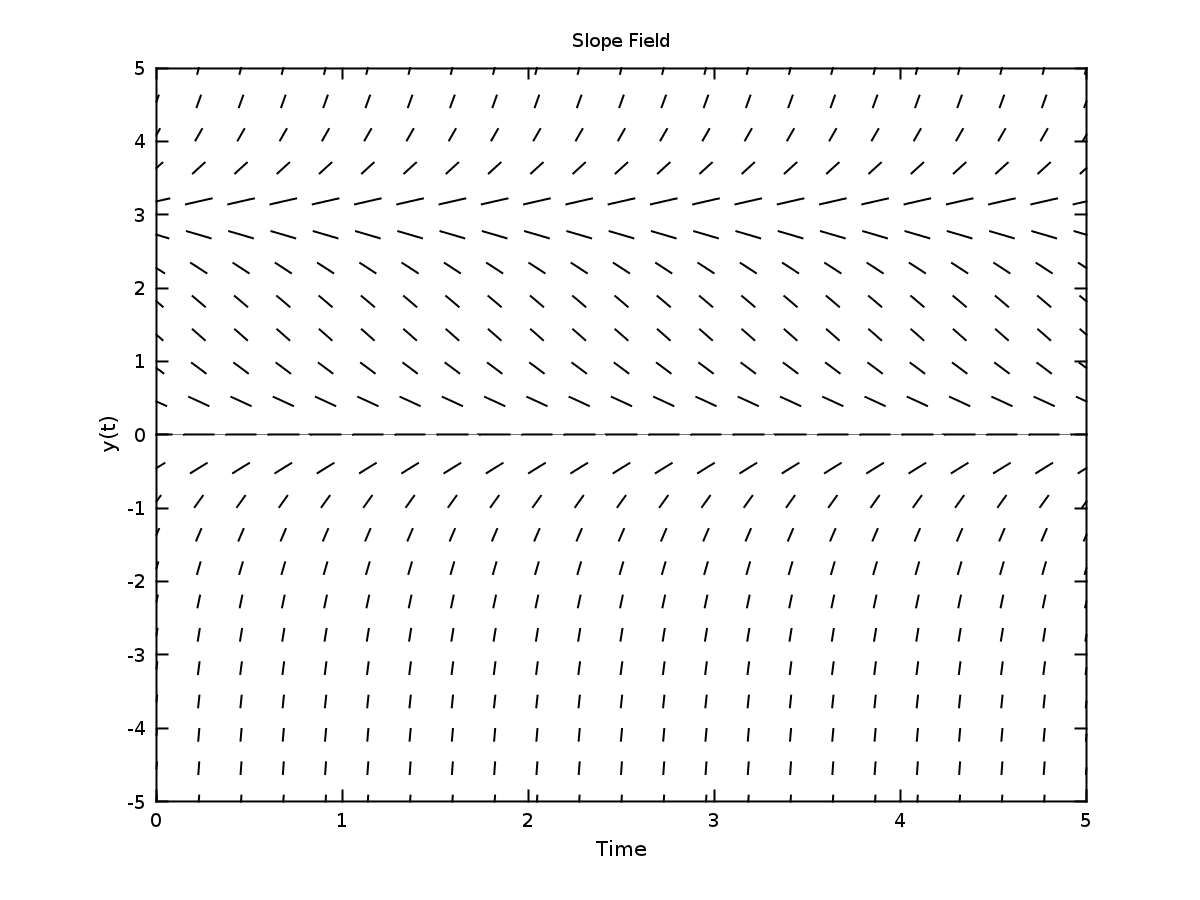
\includegraphics[height=5cm]{week1Day2SlopeField3}

  Definition: An equilibrium solution is a value for which the
  solution does not change in time.

  \uncover<2->{$y(t)=0$ and $y(t)=3$ are equilibrium solutions.}

\end{frame}

\section{Stability}

\begin{frame}
  \frametitle{Stability}

  \begin{itemize}
  \item An \textit{equilibrium solution} is \textbf{stable} if values
    of the solution tend to stay close to it as $t$ increases.
  \item An \textit{equilibrium solution} is \textbf{unstable} if
    values of the solution tend to move away from it as $t$ increases.
  \end{itemize}

  In the previous example $y=0$ is stable while $y=3$ is unstable.

\end{frame}



% LocalWords:  Clarkson pausesection hideallsubsections isocline


\part{Separable Equations}


\title{Ordinary Differential Equations}
\subtitle{Math 232 - Week 1, Day 3}

\author{Kelly Black}
\institute{Clarkson University}
\date{2 Sep 2011}

\begin{frame}
  \titlepage
\end{frame}

\begin{frame}
  \frametitle{Outline}
  \tableofcontents[pausesection,hideallsubsections]
\end{frame}


\section{The Chain Rule}


\begin{frame}
  \frametitle{Finding Solutions}

  How do we find a solution to a DE?

  \uncover<2->{Depends!}


\end{frame}


\begin{frame}
  \frametitle{The Chain Rule}

  \begin{eqnarray*}
    \int \lp 1 + \ln(t) \rp \frac{1}{t} ~ dt & = & ?
  \end{eqnarray*}

  \uncover<2->{
    Let $u=1+\ln(t)$ then $du=\frac{1}{t}.$
  }

  \uncover<3-> {
    \begin{eqnarray*}
      \int \lp 1 + \ln(t) \rp \frac{1}{t} ~ dt & = & \int u ~ du \\
      & = & \half u^2 + C \\
      & = & \half \lp 1+\ln(t) \rp^2 + C
    \end{eqnarray*}
  }


\end{frame}

\begin{frame}
  \frametitle{The Chain Rule}

  \begin{eqnarray*}
    \int \lp 1 + \ln(t) \rp \frac{1}{t} ~ dt & = & ?
  \end{eqnarray*}

  \uncover<2->{
    Let $y=1+\ln(t)$ then $dy=\frac{1}{t}.$
  }

  \uncover<3-> {
    \begin{eqnarray*}
      \int \lp 1 + \ln(t) \rp \frac{1}{t} ~ dt & = & \int y ~ dy \\
      & = & \half y^2 + C \\
      & = & \half \lp 1+\ln(t) \rp^2 + C
    \end{eqnarray*}
  }


\end{frame}

\begin{frame}
  \frametitle{The Chain Rule}
  \begin{eqnarray*}
    \int f(y) y' ~ dt & = & \int f(y) ~ dy
  \end{eqnarray*}

  So what?

\end{frame}


\begin{frame}
  \frametitle{A Differential Equation}
  
  \begin{eqnarray*}
    y' & = & 2y
  \end{eqnarray*}

  What is $y$?

  \uncover<2->{
    Note:
    \begin{eqnarray*}
      \frac{1}{y} y' & = & 2
    \end{eqnarray*}
    I can get all the ``$y$''s on the left and the ``t''s on the
    right.
  }

\end{frame}

\section{Separable Equations}

\begin{frame}
  \frametitle{Separable Equations}

  Definition: A \textbf{separable differential equation} is an
  equation that can be expressed in the form 
  \begin{eqnarray*}
    y' & = & f(t) g(y).
  \end{eqnarray*}

  In our example:
  \begin{eqnarray*}
    y' & = & 2y \\
    f(t) & = & 2 \\
    g(y) & = & y
  \end{eqnarray*}

\end{frame}


\begin{frame}
  \frametitle{Solving Our Example}

  \begin{eqnarray*}
    y' & = & 2y \\
    \frac{1}{y} y' & = & 2, \\
    \uncover<2->{
      \int \frac{1}{y} y' ~ dt & = & \int 2 ~ dt \\
      \int \frac{1}{y} ~ dy & = & \int 2 ~ dt } \\
    \uncover<3->{
      \ln(y) & = & 2t + C } \\
    \uncover<4->{
      y & = & e^{2t + C} \\
      y & = & e^{2t} \cdot e^C \\
      y & = & k e^{2t}
    }
  \end{eqnarray*}

\end{frame}


\begin{frame}
  \frametitle{In General}

  \begin{eqnarray*}
    y' & = & f(t) g(y) \\
    \frac{1}{g(y)} y' & = & f(t) \\
    \int \frac{1}{g(y)} y' ~ dt & = & \int f(t) ~ dt \\
    \int \frac{1}{g(y)} ~ dy & = & \int f(t) ~ dt 
  \end{eqnarray*}

  \begin{itemize}
  \item Solve the integrals
  \item Solve for $y$ (if possible)
  \end{itemize}


\end{frame}


\begin{frame}
  \frametitle{Example}

  \begin{eqnarray*}
    y' & = & \frac{t}{y+y^2} \\
    \uncover<2->{
      \lp y + y^2 \rp y' & = & t } \\
    \uncover<3->{
      \int \lp y + y^2 \rp y' ~ dt & = & \int t ~ dt \\
      \int \lp y + y^2 \rp ~ dy & = & \int t ~ dt } \\
    \uncover<4->{
      \half y^2 + \frac{1}{3} y^3 & = & \half t^2 + C
    }
  \end{eqnarray*}

  \uncover<5->{
    Cannot solve explicitly for $y(t)$!
  }

\end{frame}


\begin{frame}
  \frametitle{Example}

  \begin{eqnarray*}
    y' & = & 3y + t
  \end{eqnarray*}

  \uncover<2-> { Not separable! }

\end{frame}


\begin{frame}
  \frametitle{Example}

  \begin{eqnarray*}
    y' & = & y^2 + 1 \\
    \uncover<2->{
      \frac{1}{y^2 + 1} y' & = & 1 } \\
    \uncover<3->{
      \int \frac{1}{y^2 + 1} y' ~ dt  & = & \int 1 ~ dt \\
      \int \frac{1}{y^2 + 1}  ~ dy  & = & \int 1 ~ dt } \\
    \uncover<4->{
      \arctan(y) & = & t + C } \\
    \uncover<5->{
      y & = & \tan(t+C)}
  \end{eqnarray*}

\end{frame}


\begin{frame}
  \frametitle{Example}

  \begin{eqnarray*}
    y' & = & yt + t \\
    \uncover<2->{
      y' & = & t(y+1) }\\
    \uncover<3->{
      \int \frac{1}{y+1} y' ~ dt & = & \int t ~ dt \\
      \int \frac{1}{y+1} ~ dy & = & \int t ~ dt \\
    }
    \uncover<4->{
      \ln(y+1) & = & \half t^2 + C }\\
    \uncover<5->{
      y+1 & = & e^{\half t^2 + C} \\
      y+1 & = & e^{\half t^2}e^{C} \\
      y+1 & = & k e^{\half t^2} \\
      y = ke^{\half t^2} - 1 }
  \end{eqnarray*}

\end{frame}


\begin{frame}
  \frametitle{Example}

  \begin{eqnarray*}
    y' & = & \cos(ty) 
  \end{eqnarray*}

  \uncover<2->{Not Separable!}

\end{frame}


\begin{frame}
  \frametitle{Example}

  \begin{eqnarray*}
    y' & = & \frac{t}{y}, ~~~ y(0)=2 \\
    \uncover<2->{
      y y' & = & t } \\
    \uncover<3->{
      \int y y' ~ dt & = & \int t ~ dt } \\
    \uncover<4->{
      \half y^2 & = & \half t^2 + C \\
      y^2 & = & t^2 + k } \\
    \uncover<5->{
      2^2 & = & 0 + k \\
      k   & = & 4 \\
      y & = & \pm \sqrt{t^2+4} } \\
    \uncover<6->{
      \mathrm{Must ~ be ~ positive!} \\
      y & = & \sqrt{t^2+4} }
  \end{eqnarray*}

  \uncover<6->{
    See example 4 in the book.
  }

\end{frame}


\begin{frame}
  \frametitle{Example}

  \begin{eqnarray*}
    ty' & = & y^2 t^2 + 1 \\
    \uncover<2->{
      y'  & = & y^2 t + \frac{1}{t} }
  \end{eqnarray*}

  \uncover<3->{Not separable!}

\end{frame}


\begin{frame}
  \frametitle{Example}

  \begin{eqnarray*}
    t y' & = & y^2+1 \\
    \uncover<2->{
      \frac{y'}{y^2+1} & = & \frac{1}{t} } \\
    \uncover<3->{
      \int \frac{y'}{y^2+1} ~ dt & = & \int \frac{1}{t} ~ dt \\
      \int \frac{1}{y^2+1} ~ dy & = & \int \frac{1}{t} ~ dt } \\
    \uncover<4->{
      \arctan(y) & = & \ln(t)+C } \\
    \uncover<5->{
      y & = & \tan(\ln(t)+C)}
  \end{eqnarray*}





\end{frame}


\begin{frame}
  \frametitle{Example}

  \vspace*{-3em}
  \begin{eqnarray*}
    y' & = & \sec(y) t^2 + \sec(y) \sin(4t) \\
    \uncover<2->{
      y' & = & \sec(y) \lp t^2 + \sin(4t) \rp } \\
    \uncover<3->{
      \frac{y'}{\sec(y)} & = & t^2 + \sin(4t) } \\
    \uncover<4->{
      \int \frac{y'}{\sec(y)} ~ dt & = & \int t^2 + \sin(4t) ~ dt \\
      \int \frac{1}{\sec(y)} ~ dy & = & \int t^2 + \sin(4t) ~ dt }\\
    \uncover<5->{
      \int \cos(y) ~ dy & = & \int t^2 + \sin(4t) ~ dt } \\ 
    \uncover<6->{
      \sin(y) & = & \frac{1}{3} t^3 - \frac{1}{4} \cos(4t) + C } \\
    \uncover<7->{
      y & = & \arcsin\lp\frac{1}{3} t^3 - \frac{1}{4} \cos(4t) + C\rp } \\
  \end{eqnarray*}

  \uncover<8->{This is problematic!}

\end{frame}
 


% LocalWords:  Clarkson pausesection hideallsubsections




\end{document}

% LocalWords:  Clarkson pausesection hideallsubsections
